\subsection{Architettura del sistema}

\subsection{Introduzione}
\begin{flushleft}
    Alla luce delle valutazione effettuate durante l'analisi dei requisiti, abbiamo trovato conveniente strutturare la nostra app seguendo un tipo di 
    architettura client-server. I client, nel nostro caso, sono quasi sempre dei dispositivi portatili dotati di sistema operativo android (con la possibilità volendo di utilizzare emulatori da pc desktop)
    mentre il server è stato realizzato con il framework di sviluppo Spring Boot.

\end{flushleft}

\subsubsection{Client}
\begin{flushleft}
    Come già detto, il client è composto da un'applicazione android distribuita o tramite apk o tramite play store (rispetta tutti i requisiti per essere pubblicata) che mira ad offrire un'interfaccia utente semplice e pulita 
    per l'accesso agli endpoint forniti dal nostro server Spring-Boot. Come ogni app progetto nativo Android, il nostro client adotta un modello di design MVC (Model-View-Controller) e 
    in contemporanea ad un pattern Singleton che tiene traccia dell'utente loggato e si tiene aggiornato quasi in tempo reale con i dati forniti dal server.
\end{flushleft}
\vspace{0.2cm}


\subsubsection{Server}
\begin{flushleft}
    Il back-end della nostra applicazione è stato realizzato con la tecnlogia offerta da Spring Boot, un potente framework di svillupo che sfrutta Java.
    L'architettura che prevede è anch'essa a 3 livelli e prevede i seguenti componenti:
    \begin{itemize}
        \item Model: L'insieme di classi che rappresentano le entità della nostra applicazione. Le stesse sono riportate sul client, e, cosa più importate, spring mappa le classe con annotation "@entity" 1:1 con le tabelle nel db relazionale.\\
              
        \item Repository: Sfruttando il framework JPA (Java Persistence API) riusciamo a gestire persistenza e consistenza dei dati nel db in maniera quasi automatizzata. Spring ci fornisce un gran supporto in questo ambito.
        \item Controller: Qui ci va tutta la logica di controllo del server. Sono queste le classi che espongono gli end-point Rest ai client e, comunicando con le repository aggiornano i model e le tabelle nel db allo stesso tempo.
    \end{itemize}
\end{flushleft}

\begin{figure}[H]
    \centering
    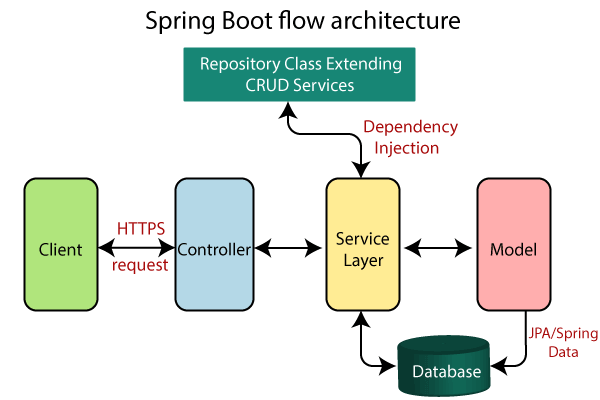
\includegraphics[scale=0.3]{assets/immagini varie/spring-boot-architecture2.png}
    \caption*{\textbf{Figura}: Spring-Boot}\label{fig:spring_Arch}
\end{figure}
\newpage

\begin{flushleft}
    \textbf{Microsoft Azure}\\
    Microsoft Azure è la piattaforma cloud pubblica di Microsoft, che offre servizi di cloud computing. Tra i vari piani che mette a disposizione, abbiamo usufruito
    di quello "gratuito" che ci permette di eseguire una macchian virtuale linux e un database relazionale, che nel nostro caso è stato PostgreSQL.
    La configurazione della macchina virtuale non ha richiesto particolari abilità: tramite connessione ssh abbiamo configurato il progetto Spring Boot e avviandolo 
    mettiamo a disposizione gli end-point raggiungibili poi dai client.
    La potenza computazionale in questa fase di sviluppo e di utilizzo limitato dell'applicativo potrebbe risultare esile, ma il vantaggio di piattaforme quali
    Azure è possibile in qualsiasi momento aumentare le risorse dedicate a db e/o macchina virtuale, aumentando di fatto la scalabilità della nostra applicazione.

\end{flushleft}